%% bare_conf.tex
%% V1.4b
%% 2015/08/26
%% by Michael Shell
%% See:
%% http://www.michaelshell.org/
%% for current contact information.
%%
%% This is a skeleton file demonstrating the use of IEEEtran.cls
%% (requires IEEEtran.cls version 1.8b or later) with an IEEE
%% conference paper.
%%
%% Support sites:
%% http://www.michaelshell.org/tex/ieeetran/
%% http://www.ctan.org/pkg/ieeetran
%% and
%% http://www.ieee.org/

%%*************************************************************************
%% Legal Notice:
%% This code is offered as-is without any warranty either expressed or
%% implied; without even the implied warranty of MERCHANTABILITY or
%% FITNESS FOR A PARTICULAR PURPOSE! 
%% User assumes all risk.
%% In no event shall the IEEE or any contributor to this code be liable for
%% any damages or losses, including, but not limited to, incidental,
%% consequential, or any other damages, resulting from the use or misuse
%% of any information contained here.
%%
%% All comments are the opinions of their respective authors and are not
%% necessarily endorsed by the IEEE.
%%
%% This work is distributed under the LaTeX Project Public License (LPPL)
%% ( http://www.latex-project.org/ ) version 1.3, and may be freely used,
%% distributed and modified. A copy of the LPPL, version 1.3, is included
%% in the base LaTeX documentation of all distributions of LaTeX released
%% 2003/12/01 or later.
%% Retain all contribution notices and credits.
%% ** Modified files should be clearly indicated as such, including  **
%% ** renaming them and changing author support contact information. **
%%*************************************************************************


% *** Authors should verify (and, if needed, correct) their LaTeX system  ***
% *** with the testflow diagnostic prior to trusting their LaTeX platform ***
% *** with production work. The IEEE's font choices and paper sizes can   ***
% *** trigger bugs that do not appear when using other class files.       ***                          ***
% The testflow support page is at:
% http://www.michaelshell.org/tex/testflow/



\documentclass[conference]{IEEEtran}

\hyphenation{op-tical net-works semi-conduc-tor}
\renewcommand{\thefootnote}{}

\IEEEoverridecommandlockouts

\usepackage{listings}


\usepackage{graphicx}
\usepackage{newlfont}
\usepackage{multicol}
\usepackage{multirow}
\usepackage[table]{xcolor}
\usepackage{tabularx}
\usepackage{cite}
\usepackage{amssymb}
\usepackage[cmex10]{amsmath}
\interdisplaylinepenalty=2500
\usepackage{array}
\usepackage{stfloats}

\usepackage{lipsum}

\usepackage{fancyhdr}
\setlength{\headheight}{15.2pt}
\pagestyle{fancy}
\renewcommand{\headrulewidth}{0.3pt}
\fancyhead{}
\chead{\textcolor[rgb]{0.5,0.5,0.5}{2017 IEEE International Young Scientists Forum on Applied Physics and Engineering} \textcolor[rgb]{0.61,0.81,0.00}{YSF-2017}}
\fancyfoot{}
\rfoot{\textcolor[rgb]{0.5,0.5,0.5}{October 17-20, 2017 | Lviv, Ukraine}}


\begin{document}

% you can use linebreaks \\ within to get better formatting as desired
\title{Designing the Database for Microarray Experiments Metadata}

% use a multiple column layout for affiliations
\author{\IEEEauthorblockN{Oleksandr Lykhenko, Alina Frolova, Maria Obolenska}
\IEEEauthorblockA{Group of Systems Biology\\Institute of Molecular Biology and Genetics of NASU\\
Kyiv, Ukraine\\
o.k.lykhenko@imbg.org.ua}}

\maketitle

\thispagestyle{fancy}



\begin{abstract}
Advancements in both computer science and biotechnology opened way for an unprecedented amount and variety of gene expression raw data to appear in the open access. It is sometimes worth to rearrange and unite data from several similar gene expression studies into new case-control groups to test new hypothesis using available data. Unfortunately, most popular gene expression databases, such as GEO and ArrayExpress, were not designed to allow these cross-study procedures. In order to locate comparable  samples in different studies numerous steps are required including gathering additional sample metadata and their standardization. Specialized databases are developed by investigators in their own fields of interest to reuse the processed data and create different case-control groups and test multiple hypothesis.

Here we present a detailed description of the specialized database creation along with its use case which is 35 gene expression cDNA microarray datasets containing expression data on more than 1000 biological samples on human placenta under conditions of preeclampsia. Samples contain sufficient metadata for them to be merged into relevant cross-experiment case-control groups for further integrative analysis.
\end{abstract}

\begin{keywords}
gene expression; database; microarray; python; postgres
\end{keywords}

\section{Background}

One of the approaches in modern molecular biology is to look at a living organism as a system of its interacting constituents (organs, tissues, cells, genes, transcripts, proteins etc.). Specifically, cDNA microarrays, hereinafter microarrays, are the technology to retrieve information about an entire profile of gene expression (activity) at a given moment of time in a biological sample of interest. As cDNA microarrays become by days cheaper and more accessible, numerous experiments are conducted and published along with experiments' raw data stored at open archive databases such as Gene Expression Omnibus (GEO) \cite{Barrett2011NCBIOn.} and ArrayExpress \cite{Rustici2013ArrayExpressTools.}. Microarray experiment raw data usually includes expression data, which gives relative numeric value of gene expression rate, and data that provide clinical and biological context for the expression data - metadata. By comparing gene expression under different clinical conditions, usually clinical case versus control group, we can get insights of how exactly do gene systems regulate themselves under given conditions.

Current database is being developed with intention to gather from ArrayExpress microarray experiments' sample metadata on human placenta under clinical condition of preeclampsia, a major pregnancy disorder. Main purpose of gathering these metadata is to reassemble samples from different but similar experiments into new larger and more statistically significant cross-experiment case-control groups of samples. Despite the fact that ArrayExpress stores metadata already, there are several reasons to maintain a database separate from ArrayExpress. First, metadata are not standardized, since they were uploaded independently and at different times in absence of common terminology naming convention. For example, the fetal gestation age can be referred as age, fetal age, fetus age (wks) and in other similar ways, and therefore gestation age for all samples in a set of experiments can not be obtained via simple search query. Second, metadata are often incomplete and insufficient for the samples to be comparable in terms of into which case or control group they should be placed.

Although our database can be used to store data on any cDNA microarray experiments or, indeed, any experiment that uses technical means to process some amount of samples, the database was designed for specific task, which is an integrative analysis of microarray experiment datasets on preeclampsia-affected human placenta.

Pre-eclampsia \cite{AboutPre21} is a disorder that occurs only during pregnancy and the postpartum period and affects both the mother and the unborn baby. Affecting at least 5-8\% of all pregnancies, it is a rapidly progressive condition characterized by high blood pressure and the presence of protein in the urine. Typically, pre-eclampsia occurs after 20 weeks of gestation (in the late 2nd or early 3rd trimesters or middle to late pregnancy) and up to six weeks postpartum (after delivery), though in rare cases it can occur earlier than 20 weeks. Globally, pre-eclampsia and other hypertensive disorders of pregnancy are a leading cause of maternal and infant illness and death. 

Although etiology and pathogenesis of pre-eclampsia are still unknown numerous studies (listed in Appendix) point at the gene dysregulation in placenta to be the cause of the disease. Besides, there are also known cases when placenta develops without fetus, called molar pregnancy \cite{MolarPregnancy}, which are associated with very early-onset pre-eclampsia. This is why we focused our study on gene expression in placenta. Finally, we chose cDNA microarray technology as most popular in pre-eclampsia studies among ones providing information on the whole transcriptome.

\section{Methods}

Our software is written in Python language using Django framework for web interface development and Postgres for relational database support. All experiment and sample metadata were automatically extracted from ArrayExpress database via Bioservices which is a Python interface to ArrayExpress. An NCBI's Gene Expression Omnibus (GEO) was used to supplement the missing data along with the corresponding scientific articles and authors personally. Medical Subject Headings (MeSH) and Experimental Factor Ontology (EFO)  were used as a standard for terminology in metadata, since MeSH is used to codify keywords in biological scientific articles and EFO is an ontology ArrayExpress itself uses while processing users' search queries.

Source code and database backup file are available at GitHub:

https://github.com/Sashkow/placenta-preeclampsia

Web interface for our database at its current stage can be accessed at:

http://194.44.31.241:24173/



\subsection{Database Schema Development}

As we are able to download from ArrayExpress metadata on experiment in general, on its microarray platform(s) and metadata on each individual sample, we may have the following entities/tables in our database: \textbf{Experiment}, \textbf{Microarray}, \textbf{Sample}. Each row is an experiment/microarray/sample and each column is a characteristic (attribute). The initial approach for the database schema is shown in Figure \ref{fig:NaiveSchema}.
\begin{figure}[!t]
        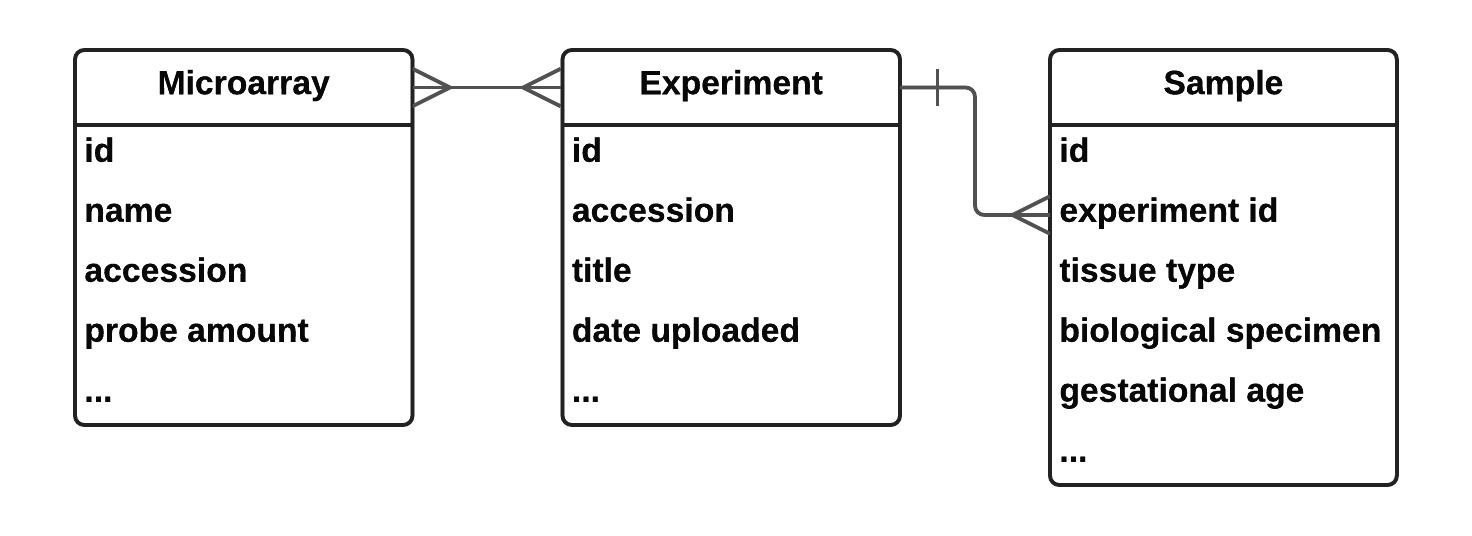
\includegraphics[width=3.5in]{plots/NaiveSchema}
        \caption{Initial database entity relation diagram}
        \label{fig:NaiveSchema}
\end{figure}

This schema is simple but will require adding new column each time new characteristic appears for either of these three entities. While Experiment and Microarray entities tend to have the characteristics uniform across ArrayExpress, the Sample entities are likely to have different set of attributes depending on Experiment they belong to. Hence, each new sample characteristic will require database schema update. Such frequent database structure updating should be avoided when possible since it may lead to incompatibility of different versions of the same database. Since, for example, not all samples will have values for all possible characteristics there will be cells in Samples table that are not filled but still taking space.

One way to resolve this issue is to replace multiple columns in a table with a single column of more complex structure. Postgres has an HStore custom field \cite{CraigKerstiensSchemalessDjango, LittImprovingBSON} which is essentially an associative array that is a collection of string key-value pairs where each key appears in the collection at most once. Replacing attributes with a single HStore field named "data" will allow adding information on new characteristics without modifying the database structure: (Figure \ref{fig:HStoreSchema}).
\begin{figure}[h] 
        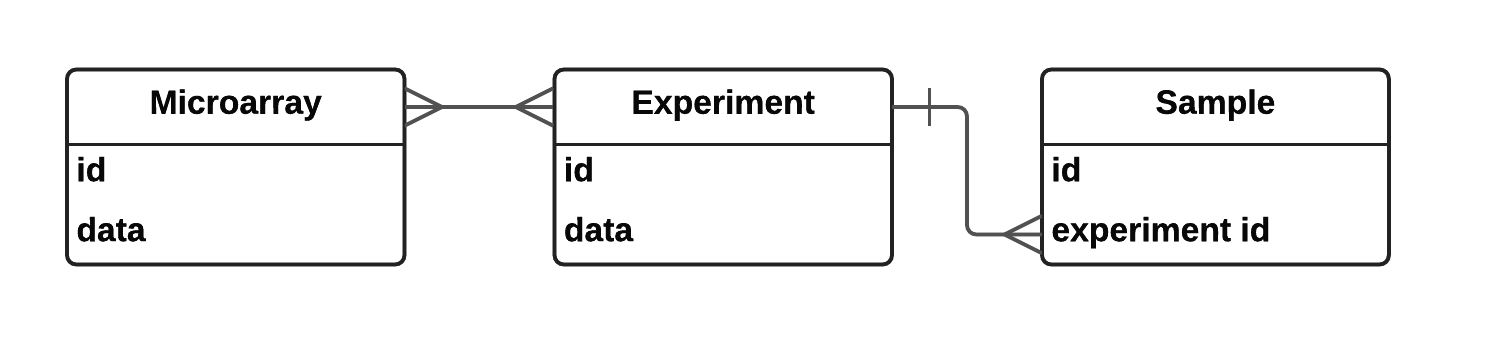
\includegraphics[width=3.5in]{plots/HStoreSchema}
        \caption{Almost schemaless database; "data" is an HStore field.}
        \label{fig:HStoreSchema}
\end{figure} 

This way if we have a sample with the attribute "age" of value "37 weeks" and the attribute "diagnosis" of value "pre-eclampsia" downloaded from ArrayExpress we store it in "data" column on Samples table equal to "{"age":"37 weeks", "diagnosis":"pre-eclampsia"}" instead of having separate columns for "age", "diagnosis" and all the other potential characteristics.

However, this implementation turns out to have disadvantages. When we downloaded our data and began sample attribute names and values standardization it occurred to us that we want to store the originally downloaded names and values along with the standardized ones. To this end, sample attributes can no longer be string name-value pairs in Sample's \textit{data} HStore dictionary field, as we now want to store four strings instead of two for each sample attribute: old name, old value, new name, new value. As a solution to this problem we replaced our "data" column with a column of indexes (foreign key) referencing a new  SampleAttribute table of all attributes for all samples. In database terminology such relation between two tables is called \textit{one-to-many relation.} SampleAttribute table in turn contains foreign keys to SampleAttributeName and SampleAttributeValue tables containing old names/values along with the new ones. (Figrue \ref{fig:KeepOldSchema})

\begin{figure}[h]
        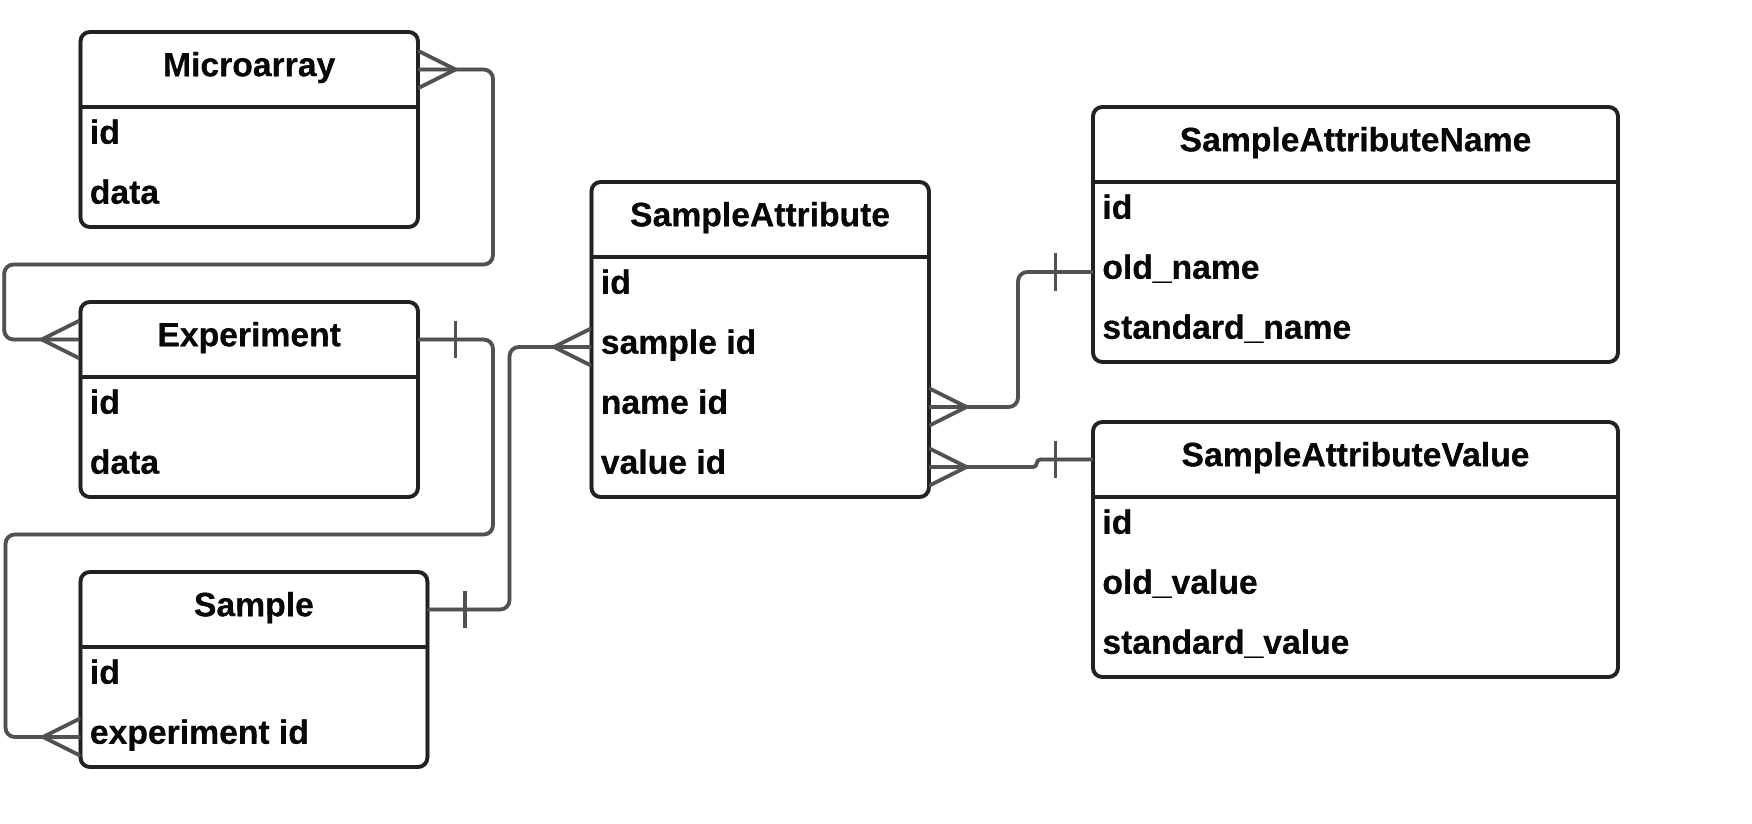
\includegraphics[width=3.5in]{plots/KeepOldSchema}
        \caption{Schema modified for keeping original values}
        \label{fig:KeepOldSchema}
\end{figure}

This schema leads to massive duplication of data because the "original-standard" mapping is ambiguous meaning that the same original name may map onto multiple standard name depending on the context of the experiment. For example, original name "placenta" may map to "Chorionic Villi" standard name if the corresponding article mentions this exact tissue type or just to "Placenta" otherwise.

In this situation it may be a good idea for standard names and values to be described once and then referred everywhere else throughout database. Old names and values, on the other hand, should be sample-attribute-related. The following schema (Figure \ref{fig:AvoidDuplicationSchema}) implements that.

\begin{figure}[h]
        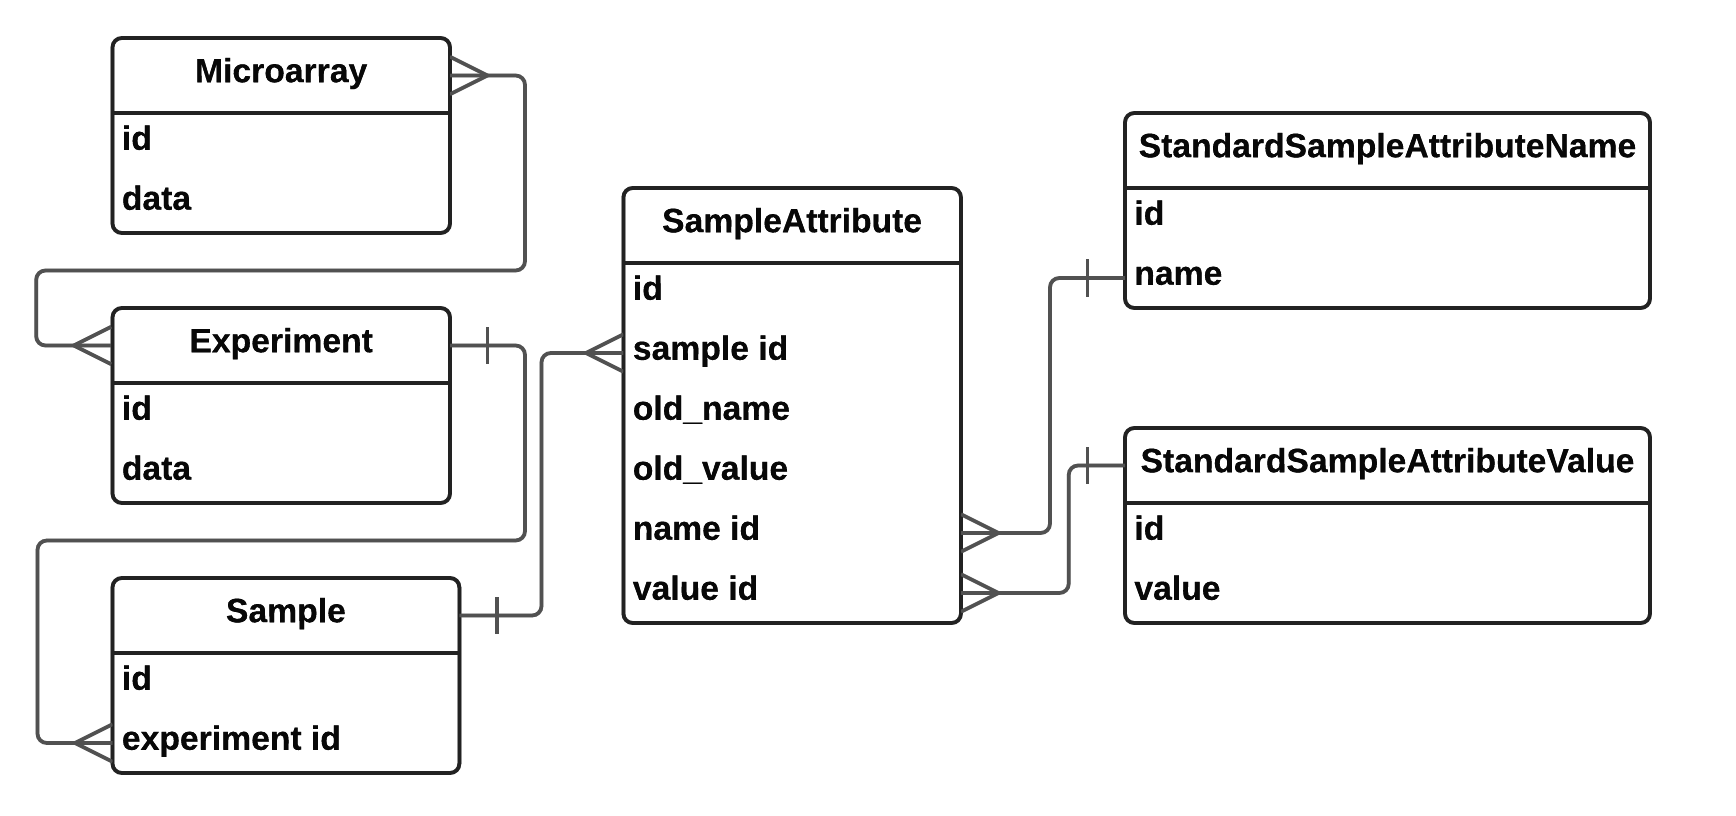
\includegraphics[width=3.5in]{plots/AvoidDuplicationSchema}
        \caption{Schema modified to avoid data duplication}
        \label{fig:AvoidDuplicationSchema}
\end{figure}

During the sample attribute standardization procedure we found out that not all original names and values can be mapped to a MeSH term as we intended. We then began to use other ontologies such as Experimental Factor Ontology (EFO) and to define our own terms. To satisfy our need in storing additional info about StandardSampleAttributeName and StandardSampleAttributeValue we added \textit{additional\_info} HStore field to these entities. To reflect the fact that some standard names and values are related either as synonyms or as parent-child we added \textit{synonyms} reflexive (to oneself) many-to-many field to StandardSampleAttributeName and StandardSampleAttributeValue entities. Finally, to show the relation between standard values and names we added one-to-many relationship from StandardSampleAttributeValue to StandardSampleAttributeName. The results are in Figure \ref{fig:FinalSchema}.

\begin{figure}[h]
        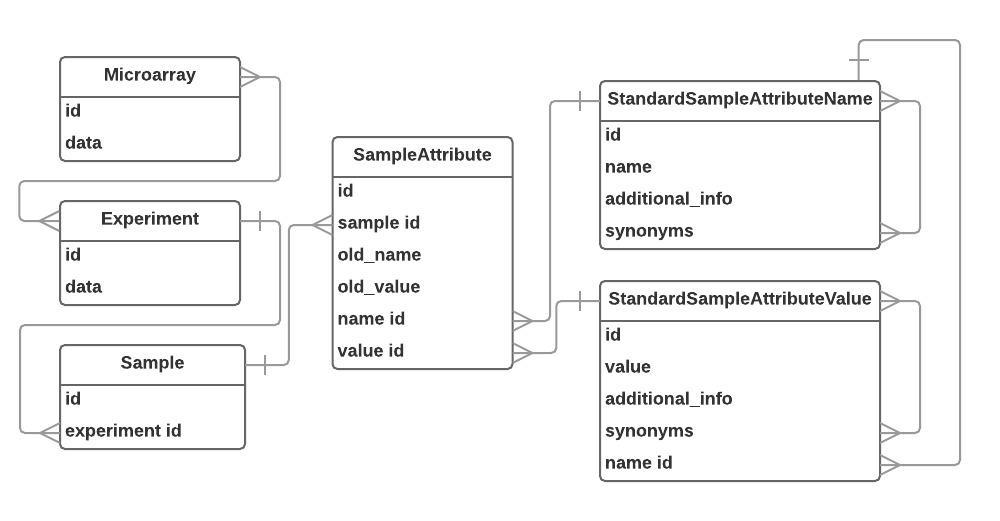
\includegraphics[width=3.5in]{plots/Schema}
        \caption{Final Schema}
        \label{fig:FinalSchema}
\end{figure}

\subsubsection{Side note}
Not all sample attribute values are qualitative with restricted list of possible values. Some of them are quantitative with numeric, textual or Boolean values. For quantitative values actual value is stored in \textit{old\_value} field while the \textit{standard\_value} specifies value type and units (like "number in weeks", "mass in grams"). Thus, a Gestation Age sample attribute may have standard\_value of Number in weeks and an old\_value of 42.

\subsubsection{Another side note}
Some attributes' original names and values were excluded from standardization process and mapped to a special standard name (or value, respectively) named "(excluded)" either due to irrelevance of the information in those attributes or because that information was moved to other attributes. Those were: "Unknown Sex", "Other", "cal id", "passage", "matching", "N/A" ect. Originally blank names and values were filled with "\textless empty\textgreater" value.

\subsection{Use case: filling database with microarray experiments on preeclampsia-affected placenta}

The initial list of 43 relevant datasets was obtained as a result of ArrayExpress search by the following query: "preeclampsia OR pre-eclampsia OR preeclamptic OR pre-eclamptic" with results filtered by organism "Homo sapiens", experiment type "rna assay", experiment type "array assay". E-GEOD-25906 was excluded due to data retrieval failure. E-MTAB-3732 was excluded since it is a compilation of microarray experiments for different diseases taken from publicly available sources. E-GEOD-15787, E-GEOD-22526, E-MEXP-1050 were excluded due to old microarray design or failure to find probe nucleotide sequences for the array. The full list of included and excluded datasets can be found in Appendix. 

From the chosen 35 (more than 1000 samples) datasets we downloaded relevant metadata and thus automatically filled Experiment, Microarray, Sample and original name-values for SampleAttribute entity. We then manually mapped original names and values to the standard ones according to well known ontologies such as MeSH and EFO \cite{MeSH,TheExper27:online}. 12\% of all sample attrubute name-value pairs were not originally present in data obtained from ArrayExpress. Missing metadata were mined from corresponding GEO datasets when such existed, from the texts of the articles using the considered datasets and from authors personally. Some datasets contained minor typos like missing link to corresponding articles or column containing data of wrong type. In such cases data update requests were sent to GEO and ArrayExpress.

While almost all datasets we retrieved from ArrayExpress are copies of corresponding datasets at GEO (group GEO), four datasets are natively from ArrayExpress (group AE). Group AE has an average of 5.9 attributes per sample versus 6.8 attributes per sample of group GEO. Group GEO has somewhat better annotation than Group AE despite being on average released later (2013.5 versus 2011.5).

\section{Results}

The database at its current stage contains a total of 32 experiment datasets and more than 1000 placenta samples, about 900 of which contain minimal metadata for relevant cross-experiment study groups to be constructed, which is diagnosis, gestational age and tissue type. The database is designed to be easily extensible to other diseases, analysis technologies, data sources and to multiple omics (as genomics, proteomics and other molecular data). The database has admin and user interfaces to search samples based on standardized metadata.

\section{Discussion}

Numerous attempts to organize gene expression data have been taken in due time including the databases we took our data from: ArrayExpress and GEO.

\textbf{G}ene \textbf{E}xpression \textbf{O}mnibus (\textbf{GEO}), an NCBI's gene expression repository founded in 2000, has a straight forward general data structure \cite{Edgar2002GeneRepository}.

\begin{figure}[h]
        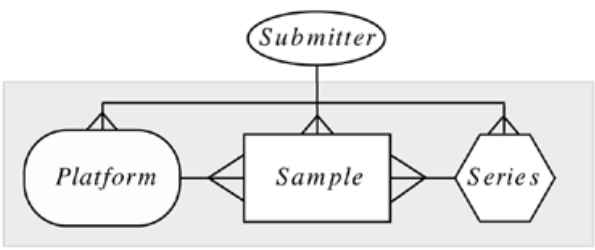
\includegraphics[width=3.5in]{plots/GeoDiagram}
        \caption{GEO entity relation diagram}
        \label{fig:GeoDiagram}
\end{figure}

\textit{Platform} entity contains a list of probes that define what set of molecules may be detected in any experiment utilizing that platform. An instance of \textit{sample} describes the derivation of the set of molecules that are being probed and utilizes platforms to generate molecular abundance data. Each sample has one, and only one, parent platform which must be previously specified. Sample may include submitter-defined clinical and other metadata concerning the sample although no standard sample attribute naming format is imposed onto submitter. \textit{Series} entity unites samples of the same experiment. It usually includes experiment related metadata such as reference to a corresponding article. 

A need for a more well-annotated experiment and sample data as well as necessity to embed external data from numerous specialized databases in accordance with already established community standards led to creation of \textbf{ArrayExpress} gene expression database in 2002. \cite{Sarkans2005ThePerspective}. Unlike GEO, database structure of ArrayExpress includes over 200 unique tables for various input data formats. Web-access on the contrary is simple and the entities accessible to user are similar to ones in GEO: experiments, samples, microarray platforms, protocols. Means of programmatic data access (also known as "application programming interface" or just API) are also available for ArrayExpress \cite{Programm69:online}. API allows retrieving detailed metadata associated with an experiment: sample annotation, protocols and data files - in XML format without need for looking through multiple tables directly.

ArrayExpress provides ability to search for specific sets of experiments depending on experiment type, submission date, studied organism, experiment description. Search query keywords are looked up in Experimental Factor Ontology to extend search with synonyms and alternative forms of the keywords (not only "pre-eclampsia", but also "preeclampsia", "pre-eclamptic"). 

A more recent \textbf{BioSamples} database has been developed focused on search for samples with similar characteristics across different experiments \cite{wwwebiac40:online}. This database, however has its own limitations due to the absence of standard sample attribute naming and to incomplete annotation, which is an obstacle to constructing cross-experiment study groups.

\textbf{GENEVESTIGATOR} is a search engine for gene expression over a compendium of manually curated datasets \cite{Hruz2008GenevestigatorTranscriptomes,ZimmermannGENEVESTIGATOR.1w,genevestigatorsite}. 
Biological samples are carefully annotated using custom ontology with a variety of characteristics allowing to filter for highly specific cases. Cross-experiment data search and analysis is based on a concept of meta-profile. As explained in \cite{Clauzel2016} meta-profiles summarize expression levels from many samples according to their biological context. Each sample is annotated with five attributes: anatomical part, cell line, cancer type, developmental stage, and perturbation - to generate meta-profiles. An exception is the Perturbation meta-profile, which consists of responses to various experimental conditions (drugs, chemicals, hormones, etc.), diseases, and genotypes. For Perturbation meta-profile results are created by comparing groups of samples from individual experiments. Data from multiple experiments are not mixed to create a single value. As a result, this tool contains large compendia of response types collected from many experiments. It also worth mentioning that samples of two different microarray platforms can not be considered simultaneously.

Another resource enabling interactive query and navigation of transcriptome datasets is \textbf{Gene Expression Browser} \cite{Speake2015AnData.} and its specific implementation for placental gene expression \cite{GXBPlacenta}. While its data are more relevant to our pursues and the interface is quite convenient and has some extended features in comparison to GEO or ArrayExpress, such as search for differentially expressed genes in a single experiment, building relevant plots, giving detailed information on found genes and and a bit of meta-analysis tools such as search for experiments that have given gene differentially expressed with a certain rate of difference, no tools for integrative analysis are provided.

\section{Conclusion}

At this time most of the samples in our database are provided with sufficient metadata for them to be comparable. These biological samples contain more complete and standardized metadata than ArrayExpress can offer and thus the samples can now constitute case-control groups of larger size than in individual datasets. Described here database will be used in forthcoming analysis, namely, the search for differentially expressed genes between different cross-experiment case and control groups. Our database is designed and expected to be enlarged with forthcoming gene expression experiments' metadata and, potentially, with other molecular biology experimental data (for example, on genome or metabolome) with relatively low effort. 

\section*{Competing interests}
The authors declare that they have no competing interests.

\section*{Author's contributions}
OL, AF designed the database. AF, MO made suggestions on database content. OL implemented database design and its admin web interface and performed metadata standardization.  All authors read and approved the final version of the article.

\bibliographystyle{bibtex/IEEEtran}
\bibliography{bibtex/IEEEabrv,bibtex/IEEEexample}

\section*{Appendix: ArrayExpress Experiments' Accesson Numbers}
Here comes the list of ArrayExpress datasets' accession numbers relevant for the search for human placenta under condition of pre-eclampsia: 'E-GEOD-74341', 'E-GEOD-73377', 'E-GEOD-73375', 'E-GEOD-73374', 'E-GEOD-60438', 'E-MTAB-3265', 'E-MTAB-3348', 'E-MTAB-3309', 'E-GEOD-54400', 'E-GEOD-59274', 'E-GEOD-57767', 'E-GEOD-48424', 'E-GEOD-57050', 'E-GEOD-54618', 'E-GEOD-49343', 'E-GEOD-38747', 'E-GEOD-47187', 'E-GEOD-50783', 'E-GEOD-41681', 'E-GEOD-44712', 'E-GEOD-44711', 'E-GEOD-44667', 'E-GEOD-43942', 'E-GEOD-41336', 'E-GEOD-41331', 'E-GEOD-40182', 'E-GEOD-37901', 'E-GEOD-36083', 'E-GEOD-35574', 'E-GEOD-31679', 'E-GEOD-30186', 'E-GEOD-15789', 'E-GEOD-15787', 'E-GEOD-22526', 'E-GEOD-24129', 'E-GEOD-10588', 'E-GEOD-13155', 'E-TABM-682', 'E-GEOD-14722', 'E-GEOD-12767', 'E-GEOD-13475', 'E-GEOD-12216', 'E-GEOD-9984', 'E-GEOD-6573', 'E-GEOD-4100', 'E-GEOD-4707', 'E-MEXP-1050'

Excluded datasets:

Could not be processed by Bioservices API: 'E-GEOD-25906'.

Irrelevant search result: 'E-MTAB-3732'

Due to microarray design: E-GEOD-15787 (Capitalbio 22K Human oligo array version 1.0, Capitalbio mammal)

E-GEOD-22526 (GynObsLU Human 800 PE-associated cDNA)

E-MEXP-1050 (Affymetrix GeneChip Human Genome Focus Array [HG-Focus])


% that's all folks
\end{document}


